\chapter{Data and bisection algorithms}


\section{Data structures}

Our first objective is to model Trieste's power grid, in order to have a computational representation on which we can develop the algorithms that mimic the restoration process and find the fault on the grid.

The dataset we use consists of some shapefiles which contain the power grid elements that are present in the \acrshort{gis} platform of the \acrshort{aaa} company. The shapefile format is a geospatial vector file format, which can also store the geometric location of an object for geographic information system (\acrshort{gis}) software. It stores the data as primitive geometric shapes, like points, lines, and polygons. Thanks to these shapes and the data attributes that are linked to each one of them (above all the position), it is possible to create the representation of the geographic data.
%In Python leggiamo questi file con la libreria GeoPandas e li salviamo in un GeoDataFrame. (?)

The company \acrshort{gis} also contains, among others, all the elements of the power grid, with different layers representing the various elements. We use the shapefile export of the layers representing the medium voltage components: electrical cables, breakers, overhead breakers, busbars, cable joints, connections, conjunctors, \acrshort{pod}s, and also of primary substations, secondary substations, and transformers.


%\section{Raw to bronze}

We proceed by refining, processing, and analyzing the data. First of all, we transform the shapefiles in Parquet files (a columnar data storage format of the Apache Hadoop ecosystem), compressing them with snappy (a fast data compression library, developed by Google and written in C++). In fact, loading and analyzing the shapefiles each time is very time-consuming, while with snappy compressed Parquet files we can really speed up the process.
% Parlare di geodf -> wkt -> parquet?

After having cleaned a bit the dataset, we remove all the elements that are flagged with something different from ``in service'' or ``out of service'' (but functioning), like ``not functioning'', or ``in construction'', or others, in order to have only the elements that are effectively used. Note that the extra cables used to create the meshed power grid are flagged as ``in service''. Since the database does not contain any information on whether a substation is remotely controlled, we have to look for it in the electrical diagrams\index{electrical diagram}, and then update the dataset accordingly. Eventually, all the remotely controlled substation and each of its breakers will be effectively flagged as remotely controlled.

We use two other pre-elaborated databases, one of which connects the \acrshort{pod}s in low voltage to their transformers, and the other computes the power in kW of each \acrshort{pod} (always in low voltage), in order to be able to compute the number of users under each transformer and the overall power of the \acrshort{pod}s.

Then we create the different data structures we need to properly model the power grid. When deciding which one would be the most appropriate, it comes natural to use graphs, since we have different elements that are connected to each other through cables. So we construct three different graphs, each refining the previous one.


%\section{Bronze to silver}

\subsection{The circuit graph}

In the first graph, we put together every component of the shapefiles, creating the \emph{circuit graph}\index{circuit graph}, which is an unrefined graph in which every electrical component of the power grid appears. It is an undirected graph since we only use it to know the connections among the various elements.

We design a class that creates the circuit graph of a power grid from the dataset, adding the nodes and the edges to the graph in the right way using the electric elements we selected. We have that the nodes are the primary and secondary substations, transformers, busbars, breakers, overhead breakers, cable joints, and \acrshort{pod}s, while the edges are electrical cables, conjunctors, and connections. We are able to connect the elements among them thanks to the dataset field \texttt{idsap}, a unique identifier that is associated with each element, and thanks to the fields that specify the connections among the components. We put in each node the useful information we have about that element, like its class (the type of object), \texttt{idsap}, code (another element identifier, but not unique --- we can see them for the substations in \autoref{fig:mastrino}), position (longitude and latitude in the WGS84 coordinate reference system, the one used by GPS coordinates), and other class-specific information, like the voltage and the number of underlying users for the transformers, or whether they are enabled for the breakers (whether they are open in the standard setup). We use a specific node for each substation, even if the substation is merely the set of its components, because we need to save the corresponding information in the graph, and this was a simple solution. Some manual modifications are needed in order to fix the graph appropriately.

After that, we create a class that simplifies a circuit graph, removing the cable joints. \emph{Cable joints}\index{cable joint} are simply used to connect two branches of a cable but, for us, they have no specific role. So, in our model, they only overburden the graph, adding more nodes that are not relevant. In fact, of around $10000$ nodes, $3000$ are cable joints. Therefore, if a cable joint simply connects two cables, we remove it, and we create a unique cable, aggregating the information of the two. We keep only those cable joints that connect three or more cables. In this way, we also remove cable joints that have only one cable attached to them, instead of two, which are dead ends.

How do we do it? We start from the complete graph, and then we prune it. We iteratively remove all the cable joints, in order to be sure of removing them all. We first create a list of nodes to be removed, which is filled with only the cable joints with node degree $2$ or less. Then we scan this list, and if a cable joint connects two cables, we aggregate the information of these edges in a new one, and we remove the joint (note that, when we remove a node, all the edges that are connected to it will be removed as well). Instead, if the node degree is less than $2$, we directly remove the joint since it is a dead end. In this way, we are able to simplify our initial graph.


\subsection{The electrical graph}

Having only the electrical components of the power grid is not sufficient, though; we also need to know the direction of the power flow. To model that, we use the \emph{electrical graph}\index{electrical graph}, which is a graph that encodes the electricity flow that passes through the elements of the circuit graph in the standard setup, when all the faulty elements are restored. Thus, it is a directed graph, since now we need to know also the specific direction of the power flow.

We construct it by first adding all the nodes of the simplified circuit graph, and then adding the edges --- which are electrical cables, conjunctors, and connections --- following the direction of the electricity flow. We start from every busbar of the primary substations, since they are the starting points of each electrical line, and we follow each connection among the elements, adding it to the graph in the right direction (pointing from the first element we encountered to the second). Since we are modeling the power flow in the standard setup, if we encounter a cable interrupted by an open breaker --- part of the ones used to create the meshed power grid --- we do not add it as an edge.
In this way, we do not introduce loops in our graph. After each edge is added (or ignored), we have finished creating our electrical graph. In \autoref{fig:secondary-substations} we can see a part of the electrical graph, in particular two secondary substations and their elements.

\begin{figure}[htbp]
    \centering
    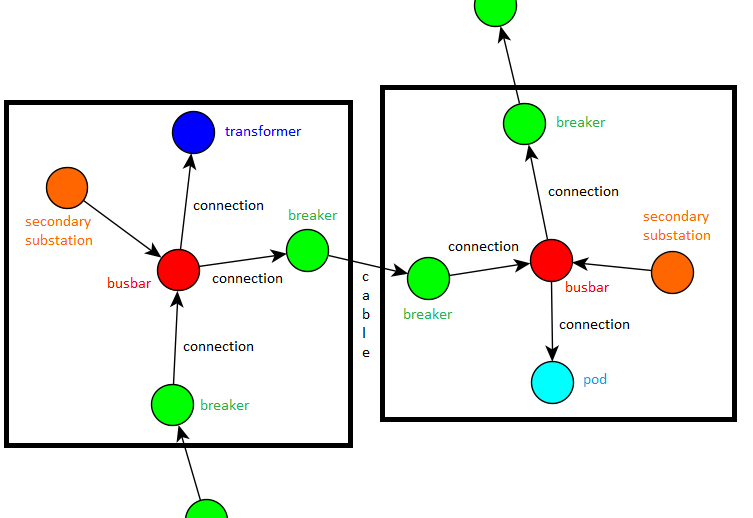
\includegraphics[scale=0.6]{chapters/figures/Secondary_substations.PNG}
    \caption{Detail of the elements of the electrical graph. We can see two secondary substations and their elements.}
    \label{fig:secondary-substations}
\end{figure}


\subsection{The substations graph}

The last graph we create is the \emph{substations graph}\index{substations graph}, a high-level, directed graph that models only the substations and their connections. We construct it by pruning the electrical graph of the other elements, so as to be able to inherit the connections among the substations and the direction of the power flow. In fact, a substation knows neither which are its elements, nor which substations are before or after itself, only its components are the ones connected among them. What we do is to cycle over all the elements, and for each type, we perform a specific action. \acrshort{pod}s and transformers can be directly removed, since they are leaves in the electrical graph, so they can be deleted easily. To remove busbars and breakers, we create a new edge between their predecessor and their successor (being careful of creating it in the right direction), named with the \texttt{idsap}s of the two nodes at its ends separated by a dash, and then we remove them, which automatically removes also the edges connected to them. If everything is done in the right way, at the end we will have the edges among the substations labeled with their \texttt{idsap}s separated by a dash, first the parent's one and then the children's one. Then we compute the number of underlying users of each substation, summing the ones of each transformer or \acrshort{pod} (in medium voltage) connected to it, and we store it in the node information.

In \autoref{fig:substations-graph} we can see a part of the substations graph, which is the computational model of the electrical diagram of \autoref{fig:mastrino}. Every node carries a lot of information about the substation, like its code, \texttt{idsap}, position, whether it is remotely controlled or not (labeled in bold and with an \texttt{R} in the figure if it is), and the number of users underneath it.

\begin{figure}[htbp]
    \centering
    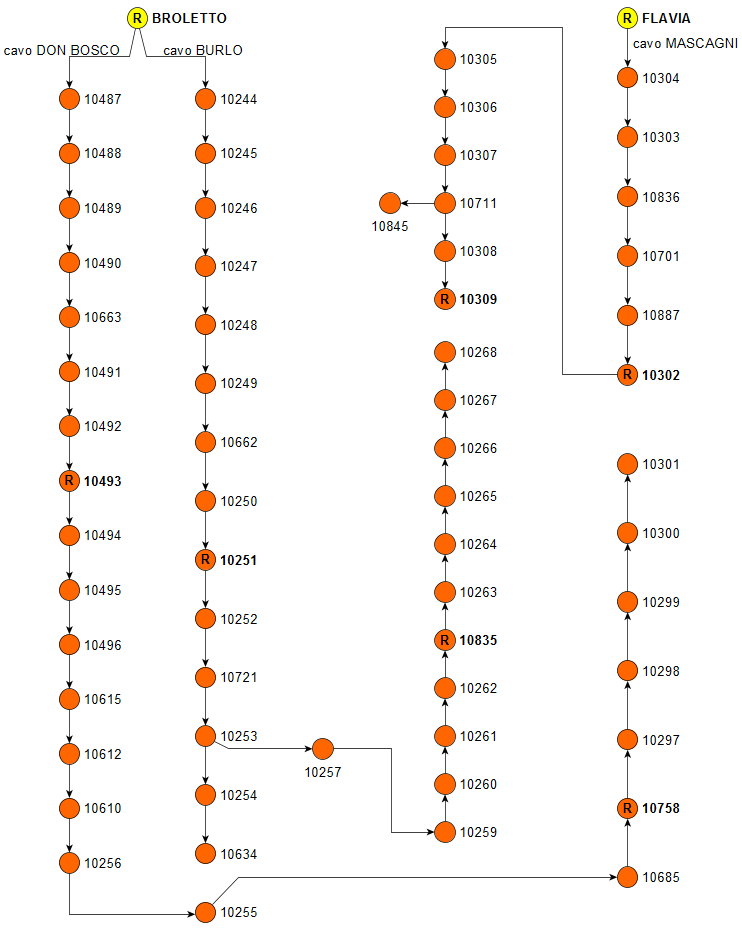
\includegraphics[scale=0.75]{chapters/figures/Substations_graph.PNG}
    \caption{Computational model of the electrical diagram of \autoref{fig:mastrino}. The substations with a bold label and with an \texttt{R} are the remotely controlled ones.}
    \label{fig:substations-graph}
\end{figure}


\section{Simulator}

The simulator is a class that creates a fault in a specific point of the power grid, or is given the position of a fault, and then using the substations graph can tell the questioner -- which will be one our algorithms --- both if the fault is before or after the current substation in which the technician is located, and how many substations can be reconnected from that substation. It encodes the information available to the technician through the different methods at their disposal to discover if the fault is before or after the substation in which they are, and the results of their actions in a substation.

To discover if the fault is before or after the currently visited substation, a function of the simulator computes the predecessors and the successors of the current substation; then it scans the graph, starting from each successor, looking for the fault, and, if it finds it, it returns the successor from which it started. If it finishes the graph, arriving in all the leaves, without finding the fault, it scans the graph from each predecessor upwards; and when it finds the fault it returns the predecessor from which it started. In this way, the simulator returns either the subsequent substation of the current one, indicating that the fault is after it, or the previous substation of the current one, indicating that the fault is before it.

Instead, to compute the list of substations that can be reconnected by operating in the current one, the function takes the output of the previous function, computes the list of predecessors of the current substation, and if the fault is in it, it starts from the current substation and visits all the subsequent ones till the end, adding all of them to a set which is returned at the end of the computation. If the fault is not in the predecessors, it is in the successors, so a traversal of the graph is made from the first remotely controlled substation until the current substation is reached, adding all these substations to a set and returning it at the end of the computation.


\section{Algorithms}


At the moment, in all our algorithms we use a simplified version of the power grid, which does not consider electrical line forks, in order to simplify the computations. Thus, we only feed our algorithms with rectilinear power lines.


\subsection{Bisection}

The bisection algorithm, which is actually a binary search algorithm, plus their experience, is what the technicians currently use to solve a fault and reconnect all the disconnected substations left out after the initial operations. We create a class that models this method, although of course not exactly, since we don't have their experience at our disposal. Our bisection algorithm, in fact, simply takes the number of currently disconnected substations and visits the one in the middle, always selecting the one on the left in case of ties. Then it uses the simulator to compute the set of remaining disconnected substations and selects another action until this set is empty. The technicians, instead, do not choose exactly the substation in the middle, but bend this rule based on many different factors, like how easy it is to enter a substation, whether it is day or night --- which also affects the first condition, the weather conditions, etcetera.


\subsection{Bisection improved}

Since the bisection algorithm, in a tie, blindly chooses the substation to the left, we were curious about how an algorithm slightly better at handling these ties would perform. So we created a bisection algorithm that, when a tie happens, chooses to visit the substation nearer to the current position of the technician. The algorithm iteratively chooses an action and uses the simulator to compute the set of remaining disconnected substations until this set is empty, which means that all the substations have been reconnected, and therefore the fault is solved.


\subsection{Weighted bisection}

The weighted bisection is yet another variation of the bisection algorithm, which determines the halfway substation to be visited according to the weights assigned to every substation. The weight of a substation is related to the cost of a fault: it is computed as the distance of the substation from the current position of the technician --- as the time it takes, in seconds, to go there --- multiplied by the number of underlying users of that substation. Thus, the algorithm computes the weight of each currently disconnected substation and decides the substation to visit by taking the one which minimizes the absolute value of the difference between the sum of the weights of the previous substations and the sum of the weights of the subsequent ones.

An efficient way to do it is to compute two vectors of the cumulated sums of the weights: one by scanning the substations from left to right, and the other one by scanning them from right to left (the latter done by flipping the initial vector, calculating the vector of the cumulated sums from left to right, and then flipping it again). Then we take the absolute value of their difference and we look for the index with the lowest value.